\documentclass[../main.tex]{subfiles}

\begin{document}

\chapter{Autoria multimídia com RA}\label{cap:proposta}

A principal contribuição deste trabalho é a proposta e avaliação de um processo de autoria baseado em realidade aumentada para a autoria de apresentações multimídia. O processo de autoria proposto é implementado na ferramenta de autoria \emph{BumbAR}, que permite a criação de conteúdo multimídia, bem como a visualização do resultado final. Além disso, a apresentação criada pode ser apresentada em navegadores de internet ou aparelhos de TV digital.

No que se segue, são discutidos o processo de autoria proposto ~(Seção~\ref{sec:processo_autoria}) e sua implementação na ferramenta \emph{BumbAR} ~(Seção~\ref{sec:implementacao_prototipo}).

\section{Processo de Autoria}
\label{sec:processo_autoria}

O processo de autoria de apresentações multimídia proposto consiste em duas fases distintas: \emph{configuração de mídias}~(Seção~\ref{subsec:midias_configuracao}), e \emph{criação de elos}~(Seção~\ref{subsec:criacao_elos}).

\subsection{Fase de configuração de mídias}
\label{subsec:midias_configuracao}

Na fase de configuração de mídias, os autores devem definir os objetos de mídia que fazem parte da apresentação e suas propriedades. Além disso, cada objeto de mídia é associado a um dos marcadores de realidade aumentada.

Um \emph{objeto de mídia} é identificado por seu \emph{nome} e pelo seu localizador de recurso uniforme, do inglês \emph{Uniform Resource Locator} (URL), que aponta para o arquivo de mídia correspondente. No contexto desta proposta, objetos de mídia englobam vídeos, imagens e áudios.

Um \emph{objeto de mídia} possui propriedades que definem como essa mídia é apresentada. Na abordagem \emph{BumbAR}, as propriedades suportadas são as comumente utilizadas em apresentações multimídia em duas dimensões, como posição na tela (x e y), tamanho (largura e altura), transparência, e volume.

Considerando as propriedades espaciais, a posição, e tamanho de \emph{objetos de mídia} são medidos em um sistema de coordenadas cartesianas 2D variando de 0 a 1, como mostrado na Figura \ref{fig:cartesiano}. A origem do sistema (0,0) é o canto inferior esquerdo da tela, e o ponto (1,1) é o canto superior direito da tela. Por exemplo, se a altura de um objeto de mídia \emph{m1} é 0.5, isso significa que a altura dele é 50\% da altura da tela.  O volume do \emph{objeto de mídia} (para áudios e vídeos) também varia de 0 a 1, onde 0 indica que o \emph{objeto de mídia} está mudo e 1 indica que seu volume está em 100\%. Além disso, a propriedade \emph{zIndex}, representado por um número inteiro, define a ordem de sobreposição de \emph{objetos de mídia}. Um \emph{objeto de mídia} com um \emph{zIndex} maior é posicionado à frente de um objeto de mídia com um valor \emph{zIndex} menor.

\begin{figure}[!h]
\centering
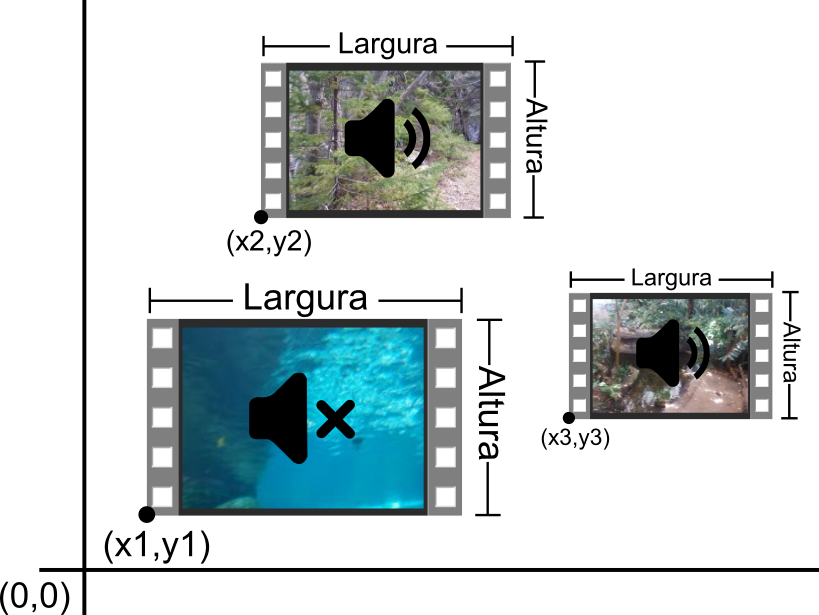
\includegraphics[width=0.7\linewidth]{IMG/media_config.png}
\caption{Configuração espacial de objetos de mídia.}
\fonte{Elaborada pelo autor.}
\label{fig:cartesiano}
\end{figure}

\subsection{Fase de criação de elos}
\label{subsec:criacao_elos}

Na fase de criação de elos, é definida a evolução da apresentação multimídia no decorrer do tempo, e como ela reage a interações do usuário. Para fazer isso, é utilizada uma interface com o usuário baseada em RA, em que marcadores de RA pré-configurados para os \emph{objetos de mídia} são dinamicamente combinados a marcadores de RA relacionados ao comportamento dos \emph{objetos de mídia} da apresentação. Tal combinação é feita por meio da colisão, no mundo real, de marcadores relacionados à \emph{objetos de mídia} com marcadores relacionados a comportamento, resultando na criação de relacionamentos entre objetos de mídia, que é detalhado a seguir. Adicionalmente, para enfatizar os diferentes marcadores e dar retorno às ações do usuário, cada marcador de realidade aumentada é renderizado como um cubo 3D, que é referenciado como \emph{Bloco RA} no restante deste trabalho.

Os relacionamentos definidos entre \emph{ojetos de mídia} seguem o modelo NCM~\cite{soares_nested_2005}. Elos (mais especificamente, elos causais) são criados a partir da colisão de \emph{blocos RA} relacionados a \emph{objetos de mídia e comportamentos}. Um elo causal determina que, quando uma uma condição é satisfeita, uma ou mais ações são executadas. Cada ação e condição suportada é representada por um marcador RA e um \emph{bloco RA} específicos.

A Tabela \ref{tab:blocos_ra} mostra exemplos de cada um dos tipos de \emph{Blocos RA} suportados. Os símbolos usados para os marcadores e \emph{Blocos RA}, entretanto, variam de acordo com a condição, ação ou \emph{objeto de mídia} específicos. Por exemplo, apesar de seguirem o mesmo modelo, o marcador e \emph{Bloco RA} de uma condição \emph{onEnd} tem um nome e símbolo diferentes de um marcador e \emph{Bloco RA} de uma condição \emph{onBegin}, mostrados na primeira linha da Tabela \ref{tab:blocos_ra}. A Tabela \ref{tab:condicoes_acoes} mostra as condições e ações individuais a serem suportadas pela ferramenta \emph{BumbAR}. Os ícones usados para cada um deles são baseados na notação visual criada por \citeonline{laiola2008visual}.

\newcommand{\imgblock}[1]{
  \raisebox{-.8\height}{\includegraphics[height=3cm]{#1}}
}

\begin{table}[!h]
\small
\caption{Os modelos de blocos de realidade aumentada da proposta BumbAR}
\label{tab:blocos_ra}
\centering
\begin{tabularx}{\linewidth}{p{3cm} X c c}

\toprule
\textbf{Tipo de bloco} & \textbf{Uso} &\textbf{Marcador RA} & \textbf{Bloco RA}
\\\otoprule
\textit{Condição}
& É usado para representar
condições.
& \imgblock{IMG/Marcadores/onBeginMarker.png}
& \imgblock{IMG/Blocos/onBeginBlock.png}
\\\midrule

\textit{Ação}
& É usado para representar ações.
& \imgblock{IMG/Marcadores/stopMarker.png}
& \imgblock{IMG/Blocos/stopBlock.png}
\\\midrule

\textit{Mídia}
& É usado para representar
\emph{objetos de mídia}.
& \imgblock{IMG/Marcadores/mediaMarker.png}
& \imgblock{IMG/Blocos/mediaBlock.png}
\\\midrule

\textit{Inicial}
& É usado para definir objetos \emph{objetos de mídia} que começam a tocar assim que a apresentação multimídia começa.
& \imgblock{IMG/Marcadores/initialMarker.png}
& \imgblock{IMG/Blocos/initialBlock.png}
\\\midrule

\textit{Deleção}
& É usado para remover elos previamente criados entre \emph{objetos de mídia}.
& \imgblock{IMG/Marcadores/delete.png}
& \imgblock{IMG/Blocos/deleteBlock.jpg}
\\\midrule
\end{tabularx}
\end{table}


\begin{table}[!h]
\small
\centering
\caption{Condições e ações usadas da proposta BumbAR.}
\label{tab:condicoes_acoes}
\begin{tabularx}{0.9\columnwidth}{ccX}
\toprule
\textbf{Nome} & \textbf{Papel} & \textbf{Significado}
\\\otoprule
onBegin       & condição     & Ativado quando o \emph{objeto de mídia} começa a tocar.
\\\midrule
onEnd         & condição     & Ativado quando o \emph{objeto de mídia} para ou acaba.
\\\midrule
onPause       & condição     & Ativado quando o \emph{objeto de mídia} é pausado.
\\\midrule
onResume      & condição     & Ativado quando o \emph{objeto de mídia} continua a ser executado depois de ter sido pausado.
\\\midrule
start         & ação        & Faz o \emph{objeto de mídia} ser iniciado.
\\\midrule
stop          & ação        & Faz o \emph{objeto de mídia} ser parado.
\\\midrule
pause         & ação        & Faz o \emph{objeto de mídia} ser pausado.
\\\midrule
resume        & ação        & Faz o \emph{objeto de mídia} continuar a tocar depois de ter sido pausado.
\\\midrule
\end{tabularx}
\end{table}

Para criar um elo causal entre dois \emph{objetos de mídia}, o usuário deve seguir os seguintes passos:

\begin{enumerate}
    \item Marcar o \emph{bloco de mídia} que é parte da condição do elo, criando um \emph{bloco de mídia-com-condição};
    \item Marcar o \emph{bloco de mídia} que é parte da ação do elo, criando um \emph{bloco de mídia-com-ação};
    \item Associar o \emph{bloco de mídia-com-condição} com o \emph{bloco de mídia-com-ação}, criando um elo causal;
\end{enumerate}

O passo 1 acima é realizado arrastando e colidindo um \emph{bloco de condição} com um \emph{bloco de mídia}. Fazendo-se isso, um ícone que representa a condição usada é adicionado ao canto superior direito do \emph{bloco de mídia}, e este torna-se um \emph{bloco de mídia-com-condição}. Um \emph{bloco de mídia-com-condição} é representado pelo mesmo \emph{bloco de mídia} que foi usado para criá-lo, mas marcado com uma condição (para fazer parte do elo). A Figura \ref{fig:midia_condicao} mostra esse processo (é possível observar que o ícone aparece no canto superior direito do \emph{bloco de mídia}).

\begin{figure}[!ht]
\centering
  \begin{subfigure}{0.49\linewidth}
    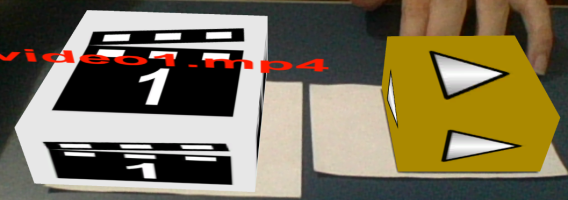
\includegraphics[width=0.95\linewidth]{IMG/beforeCondR.png}
    \caption{Antes da colisão}
  \end{subfigure}
  \begin{subfigure}{0.49\linewidth}
    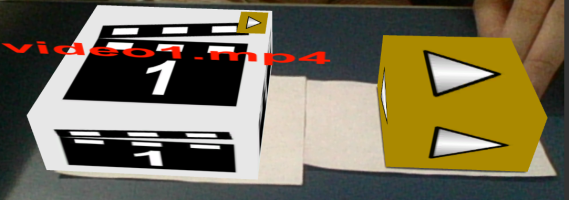
\includegraphics[width=1\linewidth]{IMG/afterCondR.png}
    \caption{Depois da colisão}
  \end{subfigure}
  \caption{\textit{Bloco de mídia} se tornando um  \textit{bloco de mídia-com-condição}}
  \fonte{Elaborado pelo autor.}
  \label{fig:midia_condicao}
\end{figure}

O passo 2, que descreve a criação de um \emph{bloco de mídia-com-ação}, segue o mesmo procedimento do \emph{bloco de mídia-com-condição}, mas fazendo-se a colisão de um \emph{bloco de mídia} com um \emph{bloco de ação}.

Depois de já ter um \emph{bloco de mídia-com-condição} ou um \emph{bloco de mídia-com-ação}, ainda é possível a alteração do tipo desse bloco. Para isso, é necessário colidir um outro \emph{bloco de condição} ou \emph{bloco de ação} com o bloco a ser alterado. Dessa forma, um mesmo \emph{objeto de mídia} pode ter diferentes papéis em diferentes elos. A Figura \ref{fig:mudando_papel} mostra um \emph{bloco de mídia-com-condição} com a condição \emph{onEnd} sendo transformado em um \emph{bloco de mídia-com-ação} com a ação \emph{Start}.

\begin{figure}[!ht]
\centering
  \begin{subfigure}{0.49\linewidth}
    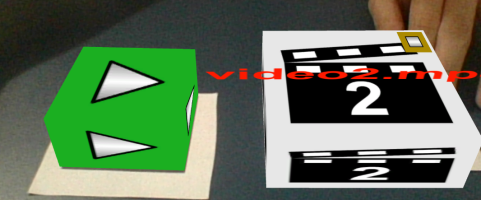
\includegraphics[width=0.95\linewidth]{IMG/beforeChangeR.png}
    \caption{Antes da colisão}
  \end{subfigure}
  \begin{subfigure}{0.49\linewidth}
    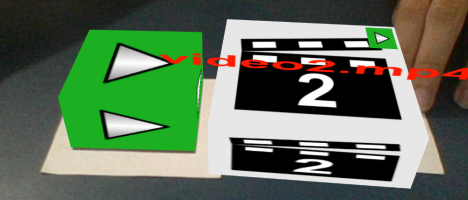
\includegraphics[width=0.95\linewidth]{IMG/afterChangeR.png}
    \caption{Depois da colisão}
  \end{subfigure}
\caption{\textit{Bloco de mídia-com-condição} se tornando um \textit{bloco de mídia-com-ação}}
\label{fig:mudando_papel}
\fonte{Elaborado pelo autor.}
\end{figure}

Finalmente, o passo 3, que descreve a criação do elo em si, é realizado por meio da colisão de um \emph{bloco de mídia-com-condição} com um \emph{bloco de mídia-com-ação}. A Figura \ref{fig:link} mostra a criação do elo \emph{onBegin mídia1 stop mídia2}.

\begin{figure}[!ht]
\centering
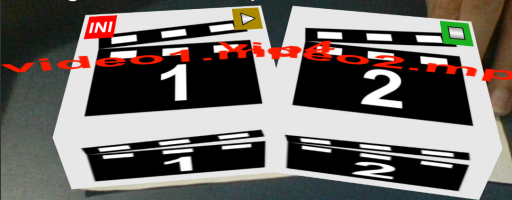
\includegraphics[width=0.6\linewidth]{IMG/linkR.png}
\caption{\textit{Elo} sendo criado}
\label{fig:link}
\fonte{Elaborado pelo autor.}
\end{figure}

A abordagem proposta também possui o \emph{bloco inicial}. Tal bloco é usado para marcar um \emph{bloco de mídia} informando que \emph{objeto de mídia} associado a ele deve ser iniciado assim que a apresentação multimídia sendo criada começar. De modo semelhante aos processos descritos anteriormente, deve-se arrastar e colidir um \emph{bloco de mídia} com o \emph{bloco inicial}. Dessa forma, um ícone com o símbolo do \emph{bloco inicial} é adicionado ao canto superior esquerdo do \emph{bloco de mídia}. A Figura \ref{fig:inicial} ilustra esse processo. Caso o usuário deseje remover este comportamento do \emph{objeto de mídia}, basta colidir novamente o \emph{bloco de mídia} correspondente com o \emph{bloco inicial}. Assim, o ícone adicionado é removido e o comportamento de iniciar assim que a apresentação começa não mais ocorre.

\begin{figure}[!h]
  \begin{subfigure}{0.49\linewidth}
    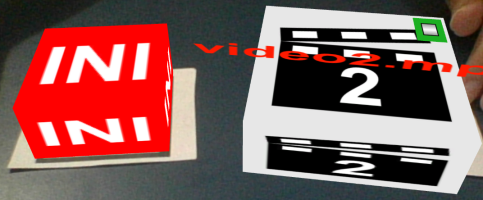
\includegraphics[width=0.95\linewidth]{IMG/beforeINIR.png}
    \caption{Antes da colisão}
  \end{subfigure}
  \begin{subfigure}{0.49\linewidth}
    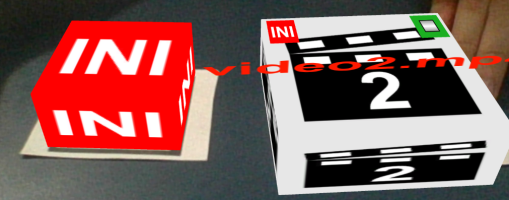
\includegraphics[width=0.95\linewidth]{IMG/afterINIR.png}
    \caption{Depois da colisão}
  \end{subfigure}
\caption{\textit{Bloco de mídia-com-ação} colide com \textit{bloco inicial}}
\label{fig:inicial}
\fonte{Elaborado pelo autor.}
\end{figure}

Além dos marcadores relacionados à blocos, o processo proposto possui dois marcadores especiais, o \emph{marcador de elos} e o \emph{marcador de visão estrutural}. Esses marcadores foram adicionados à proposta com base nos resultados colhidos do experimento que é descrito no Capítulo \ref{cap:avaliacao}.

O \emph{marcador de elos}~(Figura \ref{fig:elo}(a)) mostra, empilhados, todos os elos criados pelo usuário utilizando o processo de criação de elos descrito anteriormente. Um elo é representado pelo \emph{bloco de elo}~(Figura \ref{fig:elo}(b)). 

\begin{figure}[!h]
\centering
  \begin{subfigure}{0.3\linewidth}
  \centering
  \label{subfig:elo_marker}
    
\includegraphics[width=1\linewidth]{IMG/Marcadores/link.png}
    \caption{\textit{Marcador de elos.}}
  \end{subfigure}
  \begin{subfigure}{0.3\linewidth}
  \centering
  \label{subfig:elo_bloco}
    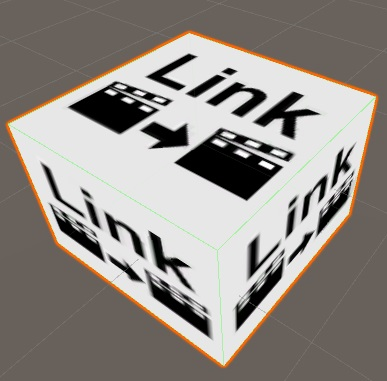
\includegraphics[width=1\linewidth]{IMG/Blocos/eloblock.jpg}
    \caption{\textit{Bloco de elo.}}
  \end{subfigure}
\caption{Marcador e bloco de elos.}
\label{fig:elo}
\fonte{Elaborado pelo autor.}
\end{figure}


Quando um \emph{bloco de elo} é renderizado, é colocado um texto sobreposto a ele representando o elo que o bloco representa, seguindo o padrão <condição> <objeto de mídia 1> <ação> <objeto de mídia 2>, de modo que quando a condição associada ao primeiro \emph{objeto de mídia} for satisfeita, a ação relacionada ao segundo \emph{objeto de mídia} será executada. Por exemplo, a Figura \ref{fig:elos} mostra o uso do \emph{marcador de elos} para mostrar dois elos criados: "\emph{onBegin media2 Stop media1}"~e "\emph{onBegin media3 Start media4}".

\begin{figure}[!ht]
\centering
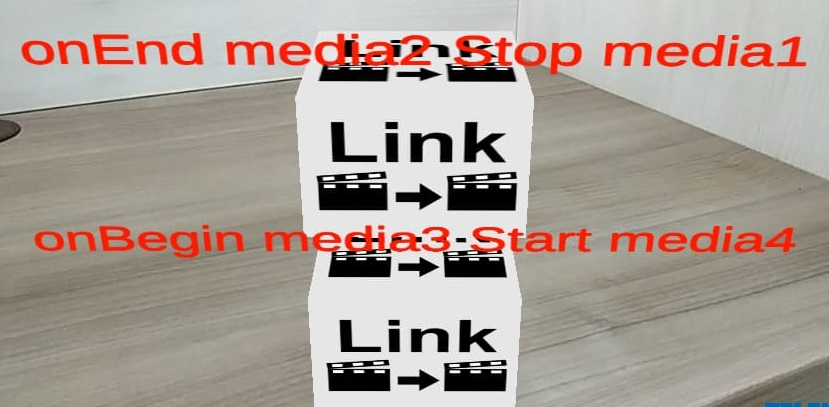
\includegraphics[width=0.6\linewidth]{IMG/Blocos/linksblock.jpg}
\caption{\textit{\emph{Blocos de elo} representando elos criados.}}
\label{fig:elos}
\fonte{Elaborado pelo autor.}
\end{figure}

Caso deseje, o usuário pode remover um elo criado. Isso evita, por exemplo, que caso um erro seja cometido durante o processo de criação da apresentação multimídia, esta não precise ser refeita do começo. Para a remoção de um elo, são usados o \emph{marcador de elos} e de \emph{deleção} em conjunto. Para efetuar a remoção do elo, o usuário deve colidir o \emph{bloco de deleção} com o \emph{bloco de elo} correspondente ao elo que deseja-se remover. A Figura \ref{fig:elo_delecao} mostra a remoção do elo "\emph{onBegin media2 Stop media1}".

\begin{figure}[!h]
  \begin{subfigure}{0.47\linewidth}
    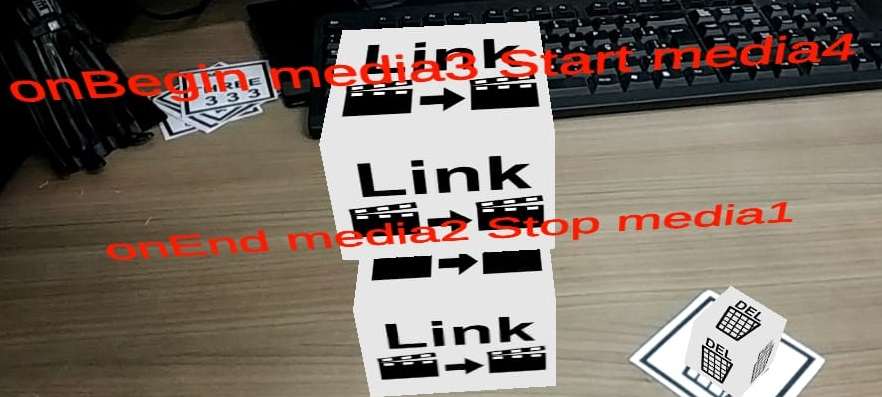
\includegraphics[width=0.95\linewidth]{IMG/delecao_antes.jpeg}
    \caption{Antes da colisão}
  \end{subfigure}
  \begin{subfigure}{0.51\linewidth}
    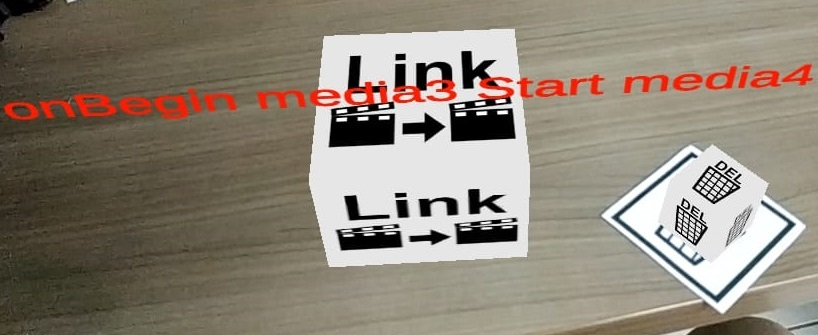
\includegraphics[width=0.95\linewidth]{IMG/delecao_depois.jpeg}
    \caption{Depois da colisão}
  \end{subfigure}
\caption{Deleção de elo.}
\label{fig:elo_delecao}
\fonte{Elaborado pelo autor.}
\end{figure}

Com o objetivo de fornecer uma visão geral da apresentação sendo criada, para que o usuário possa visualizar as relações entre \emph{objetos de mídia}, foi criado o \emph{marcador de visão estrutural}. Tal necessidade foi evidenciada a partir dos comentários dos participantes do estudo descrito no Capítulo \ref{cap:avaliacao}. Esse marcador pode ser visto na Figura \ref{fig:estrutural_marker}.

\begin{figure}[!ht]
\centering

\includegraphics[width=0.2\linewidth]{IMG/Marcadores/estrutural_marker.png}
\caption{\textit{Marcador de visão estrutural.}}
\label{fig:estrutural_marker}
\fonte{Elaborado pelo autor.}
\end{figure}

Tal marcador mostra em RA os \emph{blocos de mídia} e os elos criados entre eles de modo semelhante a um grafo, com os \emph{blocos de mídia} sendo os nós e os elos sendo as arestas. Essa visão estrutural foi inspirada na visão estrutural do NCL Composer \cite{azevedo2014composer}. A Figura \ref{fig:estrutual} mostra a visão de uma estrutural de um apresentação que possui os seguintes elos:
\begin{itemize}
    \item "\emph{onBegin media2 Stop media1}"
    \item "\emph{onBegin media3 Start media4}"
\end{itemize}

\begin{figure}[!ht]
\centering
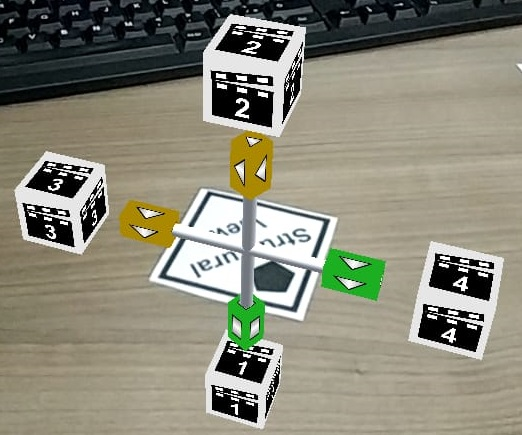
\includegraphics[width=0.45\linewidth]{IMG/estrutural.jpg}
\caption{\textit{Exemplo de visão estrutal.}}
\label{fig:estrutual}
\fonte{Elaborado pelo autor.}
\end{figure}

\section{Implementação da Ferramenta}
\label{sec:implementacao_prototipo}

A ferramenta de autoria BumbAR foi implementada como uma cena da ferramenta Unity 3D \cite{unity}. Através da reutilização de funcionalidades e objetos do Unity, a ferramenta BumbAR apresenta um ambiente tanto para a autoria, com o uso de realidade aumentada, de apresentações multimídia, quanto para tocá-las.

Tal ferramenta possui dois modos: \emph{modo de edição} e \emph{modo de apresentação}. O primeiro é o modo em que as apresentações multimídia são criadas usando o processo de autoria descrito anteriormente, e o segundo modo toca as apresentações desenvolvidas. A Figura \ref{fig:modos} destaca os dois modos e a integração destes com o ambiente do Unity.

\begin{figure}[!ht]
\centering
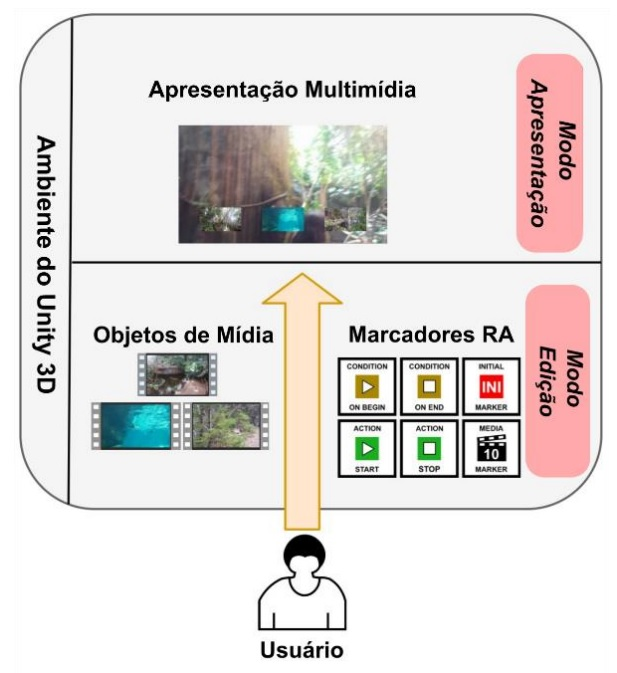
\includegraphics[width=0.45\linewidth]{IMG/modos.jpg}
\caption{\textit{Modos da ferramenta BumbAR.}}
\label{fig:modos}
\fonte{Elaborado pelo autor.}
\end{figure}

A Figura \ref{fig:componentes} mostra os componentes da ferramenta implementada. Os \emph{marcadores RA} controlam o posicionamento dos objetos de mídia, bem como dos blocos de condições, ações e demais operadores (bloco de deleção e bloco inicial). O detector de colisões é responsável pela detecção de colisões entre esses blocos. O gerenciador de elos utiliza a informação de uma colisão acontecida para, por exemplo, criar ou remover um elo. Tal gerenciamento de elos é feito de acordo com o processo descrito na Seção \ref{sec:processo_autoria}. A partir dos elos existentes, o \emph{Player} pode tocar a apresentação desenvolvida, mudando o estado da ferramenta para o \emph{modo de apresentação}. É também utilizando a informação dos elos existentes na apresentação que o \emph{NCL Parser} é utilizado para realizar a criação de um documento NCL que represente a apresentação desenvolvida. Quando o \emph{marcador de visão estrutural} está na visão da câmera, é mostrada a visão estrutural da apresentação sendo desenvolvida de acordo com os elos nela presentes.

\begin{figure}[!ht]
\centering
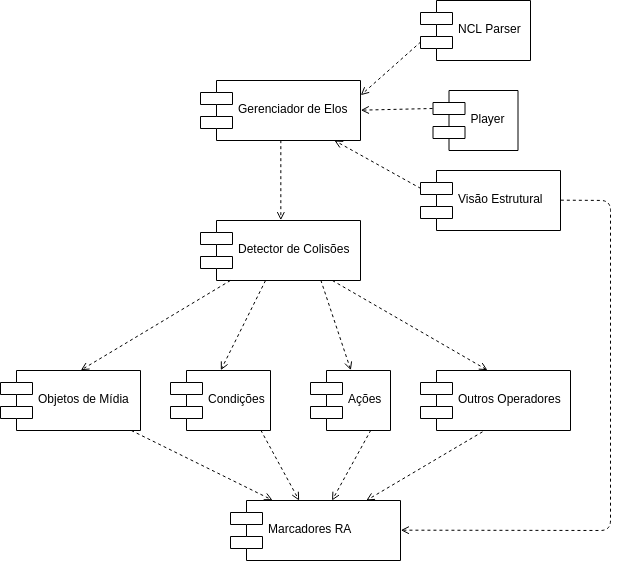
\includegraphics[width=0.65\linewidth]{IMG/componentes.png}
\caption{\textit{Componentes da ferramenta BumbAR.}}
\label{fig:componentes}
\fonte{Elaborado pelo autor.}
\end{figure}

O desenvolvimento da ferramenta foi feito em C\# \cite{hejlsberg2006c}, uma das linguagens suportadas pelo Unity 3D. Para o reconhecimento de marcadores de realidade aumentada, foi utilizado o pacote Vuforia~\cite{vuforia} para Unity 3D. Os \emph{Blocos RA}, a implementação de colisões, e controle de \emph{objetos de mídia} são feitos usando componentes nativos do Unity 3D. Eventos e métodos da linguagem C\# são usados para implementar o sistema de \emph{elos causais} utilizados na ferramenta; \emph{condições} são implementadas usando eventos da linguagem C\#, e \emph{ações} são implementadas utilizando os métodos da linguagem.

Os \emph{marcadores RA} discutidos na Seção \ref{sec:processo_autoria} são suportados na ferramenta. A adição de novos marcadores (por exemplo, para suportar todos os eventos do modelo NCM) é possível e relativamente simples para pessoas com conhecimento do funcionamento do Unity 3D. Marcadores extras podem ser criados utilizando o portal de desenvolvimento do Vuforia. Para implementar novas ações e condições, é necessário implementar seus comportamentos usando eventos e métodos da linguagem C\#.

Como mencionado anteriormente, além de tocar a apresentação multimídia criada, a ferramenta \emph{BumbAR} também suporta a exportação da apresentação para a linguagem NCL. NCL é a linguagem padrão do Sistema Brasileiro de TV Digital Terrestre \cite{abnt201115606} e recomendação ITU-T H.761 da União Internacional de Telecomunicações \cite{itu761}. Existem tocadores NCL gratuitos e comerciais tanto para TV \cite{soares_ginga-ncl_2010} e para a Web \cite{melo_webncl_2012, silva_ncl4web_2013}. Assim, uma apresentação multimídia desenvolvida utilizando a ferramenta \emph{BumbAR} também pode ser executada nesses ambientes. Como a ferramenta e a linguagem NCL usam conceitos similares provenientes do modelo NCM, como \emph{objetos de mídia} e \emph{elos causais}, exportar a representação interna da BumbAR para NCL não demandou muito esforço de implementação.


\end{document}